\documentclass[a4paper]{article}\usepackage[]{graphicx}\usepackage[]{color}
%% maxwidth is the original width if it is less than linewidth
%% otherwise use linewidth (to make sure the graphics do not exceed the margin)
\makeatletter
\def\maxwidth{ %
  \ifdim\Gin@nat@width>\linewidth
    \linewidth
  \else
    \Gin@nat@width
  \fi
}
\makeatother

\definecolor{fgcolor}{rgb}{0.345, 0.345, 0.345}
\newcommand{\hlnum}[1]{\textcolor[rgb]{0.686,0.059,0.569}{#1}}%
\newcommand{\hlstr}[1]{\textcolor[rgb]{0.192,0.494,0.8}{#1}}%
\newcommand{\hlcom}[1]{\textcolor[rgb]{0.678,0.584,0.686}{\textit{#1}}}%
\newcommand{\hlopt}[1]{\textcolor[rgb]{0,0,0}{#1}}%
\newcommand{\hlstd}[1]{\textcolor[rgb]{0.345,0.345,0.345}{#1}}%
\newcommand{\hlkwa}[1]{\textcolor[rgb]{0.161,0.373,0.58}{\textbf{#1}}}%
\newcommand{\hlkwb}[1]{\textcolor[rgb]{0.69,0.353,0.396}{#1}}%
\newcommand{\hlkwc}[1]{\textcolor[rgb]{0.333,0.667,0.333}{#1}}%
\newcommand{\hlkwd}[1]{\textcolor[rgb]{0.737,0.353,0.396}{\textbf{#1}}}%

\usepackage{framed}
\makeatletter
\newenvironment{kframe}{%
 \def\at@end@of@kframe{}%
 \ifinner\ifhmode%
  \def\at@end@of@kframe{\end{minipage}}%
  \begin{minipage}{\columnwidth}%
 \fi\fi%
 \def\FrameCommand##1{\hskip\@totalleftmargin \hskip-\fboxsep
 \colorbox{shadecolor}{##1}\hskip-\fboxsep
     % There is no \\@totalrightmargin, so:
     \hskip-\linewidth \hskip-\@totalleftmargin \hskip\columnwidth}%
 \MakeFramed {\advance\hsize-\width
   \@totalleftmargin\z@ \linewidth\hsize
   \@setminipage}}%
 {\par\unskip\endMakeFramed%
 \at@end@of@kframe}
\makeatother

\definecolor{shadecolor}{rgb}{.97, .97, .97}
\definecolor{messagecolor}{rgb}{0, 0, 0}
\definecolor{warningcolor}{rgb}{1, 0, 1}
\definecolor{errorcolor}{rgb}{1, 0, 0}
\newenvironment{knitrout}{}{} % an empty environment to be redefined in TeX

\usepackage{alltt}
\usepackage[british]{babel}
\usepackage{booktabs}
\IfFileExists{upquote.sty}{\usepackage{upquote}}{}
\begin{document}

\title{Project Report Template}
\author{Graham Williams}
\maketitle\thispagestyle{empty}

\section{Introduction}

A paragraph or two introducing the project

2015-08-25

\section{Business Problem}

Describe discussions with client (business experts) and record decisions made and share understanding of the business problem.

\section{Data Sources}

Identify the data sources and discuss acess with the data owners. Document data sources, integrity, providence, and dates.

\section{Datas Preparation}

Load the data into R and perform various operations on the the data to shape it for modelling.

\section{Data Exploration}

We should always understand our data by exploring it in various ways. Include data summaries and various plots that give insights.

\begin{kframe}
\begin{alltt}
\hlkwd{library}\hlstd{(rattle)}
\end{alltt}


{\ttfamily\noindent\itshape\color{messagecolor}{\#\# Loading required package: RGtk2\\\#\# Rattle: A free graphical interface for data mining with R.\\\#\# Version 3.5.0 Copyright (c) 2006-2015 Togaware Pty Ltd.\\\#\# Type 'rattle()' to shake, rattle, and roll your data.}}\begin{alltt}
\hlkwd{library}\hlstd{(dplyr)}
\end{alltt}


{\ttfamily\noindent\itshape\color{messagecolor}{\#\# \\\#\# Attaching package: 'dplyr'\\\#\# \\\#\# The following objects are masked from 'package:stats':\\\#\# \\\#\#\ \ \ \  filter, lag\\\#\# \\\#\# The following objects are masked from 'package:base':\\\#\# \\\#\#\ \ \ \  intersect, setdiff, setequal, union}}\begin{alltt}
\hlkwd{library}\hlstd{(xtable)}
\hlkwd{library}\hlstd{(dst)}
\hlkwd{set.seed}\hlstd{(}\hlnum{42}\hlstd{)}

\hlstd{dsname}  \hlkwb{<-} \hlstr{"weatherAUS"}
\hlstd{ds}      \hlkwb{<-} \hlkwd{tbl_df}\hlstd{(}\hlkwd{get}\hlstd{(dsname))}
\hlstd{nobs}    \hlkwb{<-} \hlkwd{nrow}\hlstd{(ds)}
\hlstd{obs}     \hlkwb{<-} \hlkwd{sample}\hlstd{(nobs,} \hlnum{5}\hlstd{)}
\hlstd{vars}    \hlkwb{<-} \hlnum{2}\hlopt{:}\hlnum{7}
\hlstd{ds}      \hlkwb{<-} \hlstd{ds[obs, vars]}
\hlstd{dst} \hlkwb{<-} \hlstd{weatherAUS[}\hlkwd{sample}\hlstd{(nobs,} \hlnum{20}\hlstd{), vars]}
\hlkwd{kable}\hlstd{(dst,} \hlkwc{row.names}\hlstd{=}\hlnum{FALSE}\hlstd{,} \hlkwc{digits}\hlstd{=}\hlnum{0}\hlstd{,} \hlkwc{booktabs}\hlstd{=}\hlnum{TRUE}\hlstd{)}
\end{alltt}
\end{kframe}
\begin{tabular}{lrrrrr}
\toprule
Location & MinTemp & MaxTemp & Rainfall & Evaporation & Sunshine\\
\midrule
Portland & 8 & 14 & 1 & 1 & 0\\
Woomera & 22 & 39 & 0 & 11 & 12\\
NorahHead & 14 & 21 & 0 & NA & NA\\
Townsville & 21 & 30 & 0 & 10 & 12\\
MountGambier & 7 & 17 & 0 & 1 & 5\\
\addlinespace
MelbourneAirport & 7 & 14 & 3 & 1 & 3\\
Nuriootpa & 12 & 18 & 2 & 9 & 9\\
Launceston & 5 & 14 & 0 & NA & NA\\
WaggaWagga & 1 & 15 & 0 & 4 & 10\\
MelbourneAirport & 12 & 17 & 1 & 9 & 1\\
\addlinespace
Launceston & 12 & 21 & 0 & NA & NA\\
Darwin & 18 & 32 & 0 & 4 & 10\\
Newcastle & NA & 20 & 78 & NA & NA\\
Melbourne & 17 & 30 & 0 & 4 & 11\\
Dartmoor & 0 & 15 & 0 & 1 & 6\\
\addlinespace
Hobart & 4 & 11 & 1 & 0 & 3\\
NorahHead & 16 & 24 & 0 & NA & NA\\
Katherine & 15 & 30 & 0 & 8 & NA\\
AliceSprings & 16 & 22 & 0 & 5 & 0\\
CoffsHarbour & 18 & 25 & 2 & NA & NA\\
\bottomrule
\end{tabular}

\begin{kframe}\begin{alltt}
\hlkwd{print}\hlstd{(}\hlkwd{xtable}\hlstd{(ds,} \hlkwc{digits} \hlstd{=} \hlnum{1}\hlstd{),} \hlkwc{include.rownames}\hlstd{=}\hlnum{FALSE}\hlstd{)}
\end{alltt}
\end{kframe}% latex table generated in R 3.2.1 by xtable 1.7-4 package
% Tue Aug 25 19:46:16 2015
\begin{table}[ht]
\centering
\begin{tabular}{lrrrrr}
  \hline
Location & MinTemp & MaxTemp & Rainfall & Evaporation & Sunshine \\ 
  \hline
Hobart & 12.4 & 21.8 & 0.2 & 5.0 & 9.6 \\ 
  Launceston & 9.0 & 15.3 & 6.5 &  &  \\ 
  Williamtown & 9.3 & 20.3 & 0.8 & 3.6 & 10.3 \\ 
  PerthAirport & 6.9 & 19.8 & 0.0 & 2.2 & 9.4 \\ 
  GoldCoast & 17.7 & 27.2 & 1.0 &  &  \\ 
   \hline
\end{tabular}
\end{table}
\begin{kframe}\begin{alltt}
\hlstd{ds} \hlkwb{<-} \hlstd{dst}
\hlstd{dst[}\hlopt{-}\hlnum{1}\hlstd{]} \hlkwb{<-} \hlkwd{sample}\hlstd{(}\hlnum{10000}\hlopt{:}\hlnum{99999}\hlstd{,} \hlkwd{nrow}\hlstd{(dst))} \hlopt{*} \hlstd{dst[}\hlopt{-}\hlnum{1}\hlstd{]}
\hlkwd{print}\hlstd{(}\hlkwd{xtable}\hlstd{(dst,} \hlkwc{digits} \hlstd{=} \hlnum{0}\hlstd{),}
      \hlkwc{include.rownames}\hlstd{=}\hlnum{FALSE}\hlstd{,}
      \hlkwc{format.args}\hlstd{=}\hlkwd{list}\hlstd{(}\hlkwc{big.mark}\hlstd{=}\hlstr{","}\hlstd{))}
\end{alltt}
\end{kframe}% latex table generated in R 3.2.1 by xtable 1.7-4 package
% Tue Aug 25 19:46:16 2015
\begin{table}[ht]
\centering
\begin{tabular}{lrrrrr}
  \hline
Location & MinTemp & MaxTemp & Rainfall & Evaporation & Sunshine \\ 
  \hline
Portland & 450,232 & 771,022 & 45,023 & 33,767 & 28,140 \\ 
  Woomera & 988,062 & 1,750,540 & 0 & 478,240 & 541,404 \\ 
  NorahHead & 1,272,045 & 1,921,794 & 0 &  &  \\ 
  Townsville & 1,034,635 & 1,511,772 & 0 & 492,205 & 612,745 \\ 
  MountGambier & 588,135 & 1,431,982 & 0 & 102,284 & 451,756 \\ 
  MelbourneAirport & 542,291 & 1,092,220 & 229,137 & 76,379 & 206,223 \\ 
  Nuriootpa & 987,581 & 1,510,418 & 165,980 & 713,714 & 755,209 \\ 
  Launceston & 233,620 & 624,485 & 0 &  &  \\ 
  WaggaWagga & 57,327 & 1,089,217 & 0 & 286,636 & 745,254 \\ 
  MelbourneAirport & 127,367 & 179,142 & 14,497 & 91,124 & 9,320 \\ 
  Launceston & 1,044,934 & 1,818,016 & 0 &  &  \\ 
  Darwin & 187,598 & 344,286 & 0 & 46,900 & 107,656 \\ 
  Newcastle &  & 573,720 & 2,226,034 &  &  \\ 
  Melbourne & 1,520,261 & 2,774,935 & 0 & 384,644 & 1,016,560 \\ 
  Dartmoor & 0 & 995,280 & 26,020 & 52,041 & 422,832 \\ 
  Hobart & 194,278 & 498,940 & 52,985 & 17,662 & 141,293 \\ 
  NorahHead & 777,550 & 1,171,246 & 0 &  &  \\ 
  Katherine & 200,520 & 394,356 & 0 & 106,944 &  \\ 
  AliceSprings & 1,590,896 & 2,137,462 & 0 & 468,485 & 0 \\ 
  CoffsHarbour & 879,282 & 1,240,765 & 87,928 &  &  \\ 
   \hline
\end{tabular}
\end{table}
\begin{kframe}\begin{alltt}
\hlkwd{print}\hlstd{(}\hlkwd{xtable}\hlstd{(ds,}
             \hlkwc{digits} \hlstd{=} \hlnum{0}\hlstd{,}
             \hlkwc{caption}\hlstd{=}\hlstr{"Selected observations from \textbackslash{}\textbackslash{}textbf\{weatherAUS\}."}\hlstd{),}
      \hlkwc{include.rownames}\hlstd{=}\hlnum{FALSE}\hlstd{)}
\end{alltt}
\end{kframe}% latex table generated in R 3.2.1 by xtable 1.7-4 package
% Tue Aug 25 19:46:16 2015
\begin{table}[ht]
\centering
\begin{tabular}{lrrrrr}
  \hline
Location & MinTemp & MaxTemp & Rainfall & Evaporation & Sunshine \\ 
  \hline
Portland & 8 & 14 & 1 & 1 & 0 \\ 
  Woomera & 22 & 39 & 0 & 11 & 12 \\ 
  NorahHead & 14 & 21 & 0 &  &  \\ 
  Townsville & 21 & 30 & 0 & 10 & 12 \\ 
  MountGambier & 7 & 17 & 0 & 1 & 5 \\ 
  MelbourneAirport & 7 & 14 & 3 & 1 & 3 \\ 
  Nuriootpa & 12 & 18 & 2 & 9 & 9 \\ 
  Launceston & 5 & 14 & 0 &  &  \\ 
  WaggaWagga & 1 & 15 & 0 & 4 & 10 \\ 
  MelbourneAirport & 12 & 17 & 1 & 9 & 1 \\ 
  Launceston & 12 & 21 & 0 &  &  \\ 
  Darwin & 18 & 32 & 0 & 4 & 10 \\ 
  Newcastle &  & 20 & 78 &  &  \\ 
  Melbourne & 17 & 30 & 0 & 4 & 11 \\ 
  Dartmoor & 0 & 15 & 0 & 1 & 6 \\ 
  Hobart & 4 & 11 & 1 & 0 & 3 \\ 
  NorahHead & 16 & 24 & 0 &  &  \\ 
  Katherine & 15 & 30 & 0 & 8 &  \\ 
  AliceSprings & 16 & 22 & 0 & 5 & 0 \\ 
  CoffsHarbour & 18 & 25 & 2 &  &  \\ 
   \hline
\end{tabular}
\caption{Selected observations from \textbf{weatherAUS}.} 
\end{table}
\begin{kframe}\begin{alltt}
\hlkwd{print}\hlstd{(}\hlkwd{xtable}\hlstd{(ds,}
             \hlkwc{digits} \hlstd{=} \hlnum{0}\hlstd{,}
             \hlkwc{caption}\hlstd{=}\hlstr{"Selected observations from \textbackslash{}\textbackslash{}textbf\{weatherAUS\}."}\hlstd{,}
             \hlkwc{label}\hlstd{=}\hlstr{"MyTable"}\hlstd{),}
      \hlkwc{include.rownames}\hlstd{=}\hlnum{FALSE}\hlstd{)}
\end{alltt}
\end{kframe}% latex table generated in R 3.2.1 by xtable 1.7-4 package
% Tue Aug 25 19:46:16 2015
\begin{table}[ht]
\centering
\begin{tabular}{lrrrrr}
  \hline
Location & MinTemp & MaxTemp & Rainfall & Evaporation & Sunshine \\ 
  \hline
Portland & 8 & 14 & 1 & 1 & 0 \\ 
  Woomera & 22 & 39 & 0 & 11 & 12 \\ 
  NorahHead & 14 & 21 & 0 &  &  \\ 
  Townsville & 21 & 30 & 0 & 10 & 12 \\ 
  MountGambier & 7 & 17 & 0 & 1 & 5 \\ 
  MelbourneAirport & 7 & 14 & 3 & 1 & 3 \\ 
  Nuriootpa & 12 & 18 & 2 & 9 & 9 \\ 
  Launceston & 5 & 14 & 0 &  &  \\ 
  WaggaWagga & 1 & 15 & 0 & 4 & 10 \\ 
  MelbourneAirport & 12 & 17 & 1 & 9 & 1 \\ 
  Launceston & 12 & 21 & 0 &  &  \\ 
  Darwin & 18 & 32 & 0 & 4 & 10 \\ 
  Newcastle &  & 20 & 78 &  &  \\ 
  Melbourne & 17 & 30 & 0 & 4 & 11 \\ 
  Dartmoor & 0 & 15 & 0 & 1 & 6 \\ 
  Hobart & 4 & 11 & 1 & 0 & 3 \\ 
  NorahHead & 16 & 24 & 0 &  &  \\ 
  Katherine & 15 & 30 & 0 & 8 &  \\ 
  AliceSprings & 16 & 22 & 0 & 5 & 0 \\ 
  CoffsHarbour & 18 & 25 & 2 &  &  \\ 
   \hline
\end{tabular}
\caption{Selected observations from \textbf{weatherAUS}.} 
\label{MyTable}
\end{table}
\begin{kframe}\begin{alltt}
\hlkwd{print}\hlstd{(}\hlkwd{xtable}\hlstd{(ds,}
             \hlkwc{digits}\hlstd{=}\hlnum{0}\hlstd{,}
             \hlkwc{caption}\hlstd{=}\hlkwd{paste}\hlstd{(}\hlstr{"Here we include a cample f \textbackslash{}\textbackslash{}LaTeX\{\}"}\hlstd{,}
                           \hlstr{"symbols that can be included in the string"}\hlstd{,}
                           \hlstr{"for example"}\hlstd{,}
                           \hlstr{"$\textbackslash{}\textbackslash{}alpha$ $\textbackslash{}\textbackslash{}longrightarrow$ $\textbackslash{}\textbackslash{}wp$."}\hlstd{,}
                           \hlkwd{Sys.time}\hlstd{()),}
             \hlkwc{lable}\hlstd{=}\hlstr{"SymbolCaption"}\hlstd{),}
      \hlkwc{include.rownames}\hlstd{=}\hlnum{FALSE}\hlstd{)}
\end{alltt}
\end{kframe}% latex table generated in R 3.2.1 by xtable 1.7-4 package
% Tue Aug 25 19:46:16 2015
\begin{table}[ht]
\centering
\begin{tabular}{lrrrrr}
  \hline
Location & MinTemp & MaxTemp & Rainfall & Evaporation & Sunshine \\ 
  \hline
Portland & 8 & 14 & 1 & 1 & 0 \\ 
  Woomera & 22 & 39 & 0 & 11 & 12 \\ 
  NorahHead & 14 & 21 & 0 &  &  \\ 
  Townsville & 21 & 30 & 0 & 10 & 12 \\ 
  MountGambier & 7 & 17 & 0 & 1 & 5 \\ 
  MelbourneAirport & 7 & 14 & 3 & 1 & 3 \\ 
  Nuriootpa & 12 & 18 & 2 & 9 & 9 \\ 
  Launceston & 5 & 14 & 0 &  &  \\ 
  WaggaWagga & 1 & 15 & 0 & 4 & 10 \\ 
  MelbourneAirport & 12 & 17 & 1 & 9 & 1 \\ 
  Launceston & 12 & 21 & 0 &  &  \\ 
  Darwin & 18 & 32 & 0 & 4 & 10 \\ 
  Newcastle &  & 20 & 78 &  &  \\ 
  Melbourne & 17 & 30 & 0 & 4 & 11 \\ 
  Dartmoor & 0 & 15 & 0 & 1 & 6 \\ 
  Hobart & 4 & 11 & 1 & 0 & 3 \\ 
  NorahHead & 16 & 24 & 0 &  &  \\ 
  Katherine & 15 & 30 & 0 & 8 &  \\ 
  AliceSprings & 16 & 22 & 0 & 5 & 0 \\ 
  CoffsHarbour & 18 & 25 & 2 &  &  \\ 
   \hline
\end{tabular}
\caption{Here we include a cample f \LaTeX{} symbols that can be included in the string for example $\alpha$ $\longrightarrow$ $\wp$. 2015-08-25 19:46:16} 
\end{table}


\begin{knitrout}
\definecolor{shadecolor}{rgb}{0.969, 0.969, 0.969}\color{fgcolor}
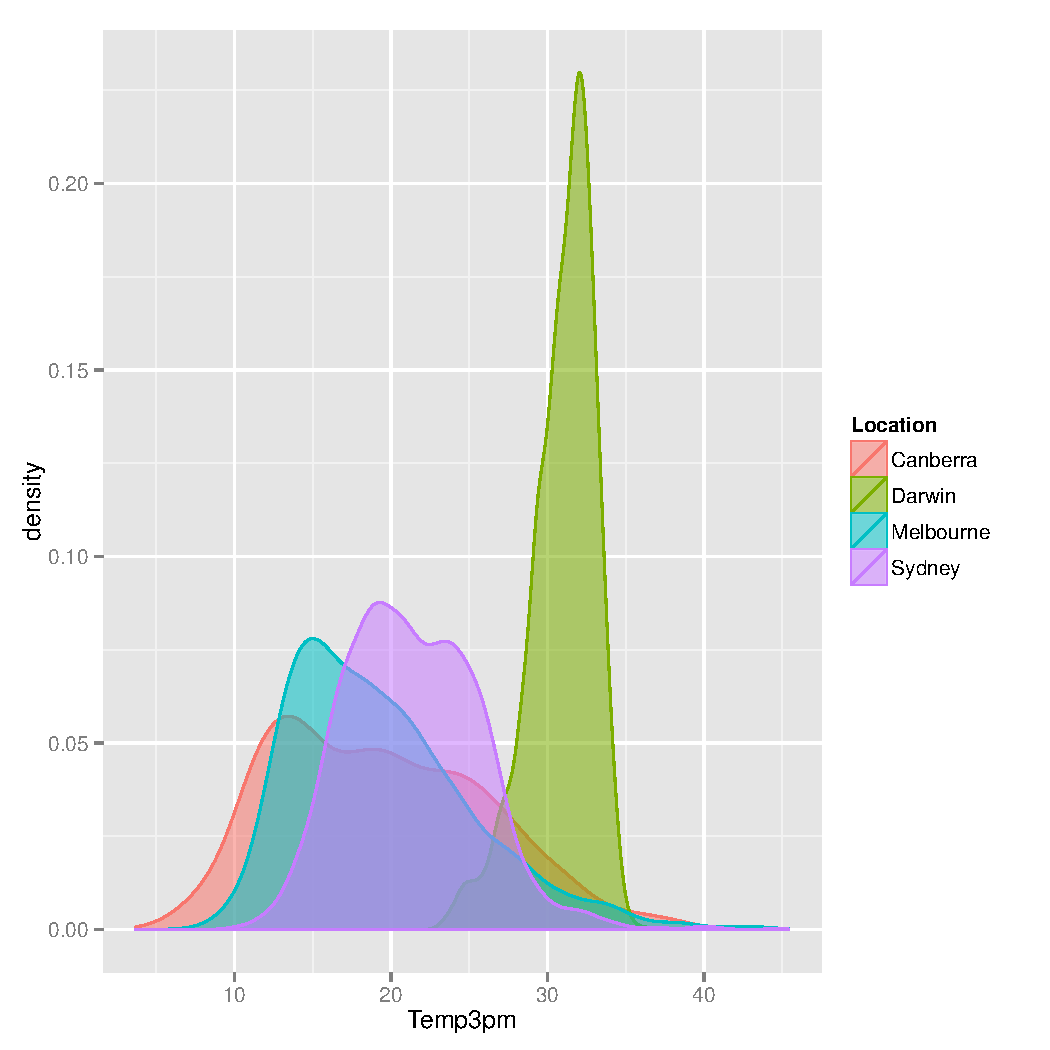
\includegraphics[width=\maxwidth]{figure/myfigure-1} 

\end{knitrout}

\begin{knitrout}
\definecolor{shadecolor}{rgb}{0.969, 0.969, 0.969}\color{fgcolor}
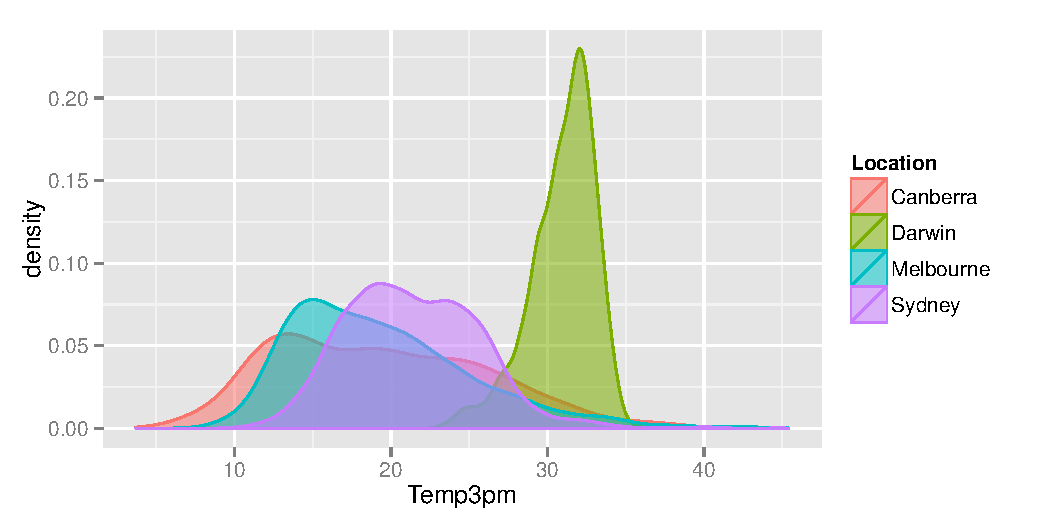
\includegraphics[width=\maxwidth]{figure/myfigure2-1} 

\end{knitrout}
\section{Model Building}

Include all models built and parameters tried. Include R code and model evaluations.

\section{Deployment}

Choose the model to deploy and export it, perhaps as PMML.

\end{document}
